% !TeX root = ../main.tex

% inserire da qualche parte (capire se mglio all'inizio per tutti i moduli oppure in ogni implementazione dei moduli)
% le configurazioni dei tool necessarie per lo sviluppo kmm e la ci: come gradle, plugin, detekt, sonar, sqldelight ecc

\section{Introduzione}
Dato il processo di sviluppo e configurato il sistema di automazione è possibile partire con lo sviluppo effettivo della applicazione mobile multipiattaforma MaggioliEbook. In questo capitolo vengono descritte le fasi di progettazione e implementazione di una applicazione mobile tramite l'utilizzo del framework Kotlin Multiplatform Mobile, rispettando i requisiti definiti nel capitolo \ref{ch:casodistudio}.

\section{Progettazione}
La fase di progettazione, come anticipato nel capitolo \ref{ch:sdlc}, comprende diverse attività tra cui le principali sono (\textit{i}) la modellazione del dominio, (\textit{ii})la progettazione dell'interfaccia grafica/esperienza utente tramite l'ausilio di mockup e (\textit{iii}) la progettazione della architettura.

\subsection{Modellazione del dominio}
Seguendo la cultura Domain-Driven Design adottata per la raccolta dei requisiti e per la definizione dei casi d'uso e della terminologia è necessario individuare i differenti contesti al fine di realizzare una mappa, detta \textit{Context Map}, utile a dare una visione globale del progetto e delle relazioni tra i vari contesti~\cite{evans_domain-driven_2004}.

La context map è composta dai seguenti tre contesti:

\begin{itemize}
    \item \textbf{Reader} (Core) - Contesto principale del progetto. Racchiude tutti gli aspetti con maggiore valore per l'utente riguardanti la lettura e la personalizzazione dei contenuti digitali. 
    \item \textbf{Sisred} - Rappresenta il contesto della sorgente dei contenuti digitali Maggioli. In questo contesto non esistono i concetti di \textit{favorite}, \textit{highlight}, \textit{bookmark} e \textit{progression} mentre è condiviso il concetto di libro e utente.
    \item \textbf{User} - Contesto che definisce tutti gli aspetti a riguardo degli utenti. In questo contesto esiste il solo concetto di utente, il quale è condiviso con gli altri contesti.
\end{itemize}

\begin{figure}[H]
    \centering
    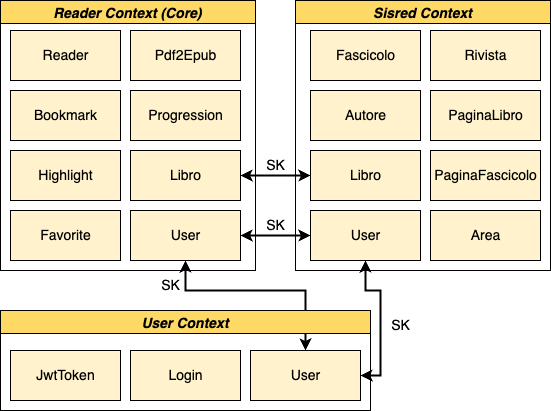
\includegraphics[width=0.8\textwidth]{img/ddd-context-map.png}
    \caption{Panoramica globale dei contesti del progetto e delle relazioni che intercorrono tra di essi}
\end{figure}

Tra i contesti definiti esistono delle relazioni di tipo \textit{Shared Kernel}~\cite{evans_domain-driven_2004} (SK) con l'obiettivo di evitare duplicazioni e semplificare l'integrazione. Relazioni di questo tipo consistono nella condivisione di un sottoinsieme del dominio modellato, che corrisponde tipicamente al dominio core. Un esempio di relazione SK è l'utilizzo di codice o schemi DB condivisi\footnote{\href{https://github.com/ddd-crew/context-mapping}{https://github.com/ddd-crew/context-mapping}}.

Per la modellazione del dominio si fa uso dei seguenti concetti\cite{evans_domain-driven_2004}:
\begin{itemize}
    \item \textbf{Entity} - Oggetto definito dalla sua identità e non dai suoi attributi. Ogni libro è univoco, identificato da uno specifico codice, chiamato ISBN\footnote{International Standard Book Number}.
    \item \textbf{Value Object} - Al contrario delle entità, questi oggetti sono definiti dai loro attributi e non hanno una identità concettuale ma servono a descrivere alcune caratteristiche di un oggetto. Un esempio è il segnalibro: ciò che è rilevante è la pagina del libro che esso referenzia e non la sua identità.

    \begin{figure}[H]
        \centering
        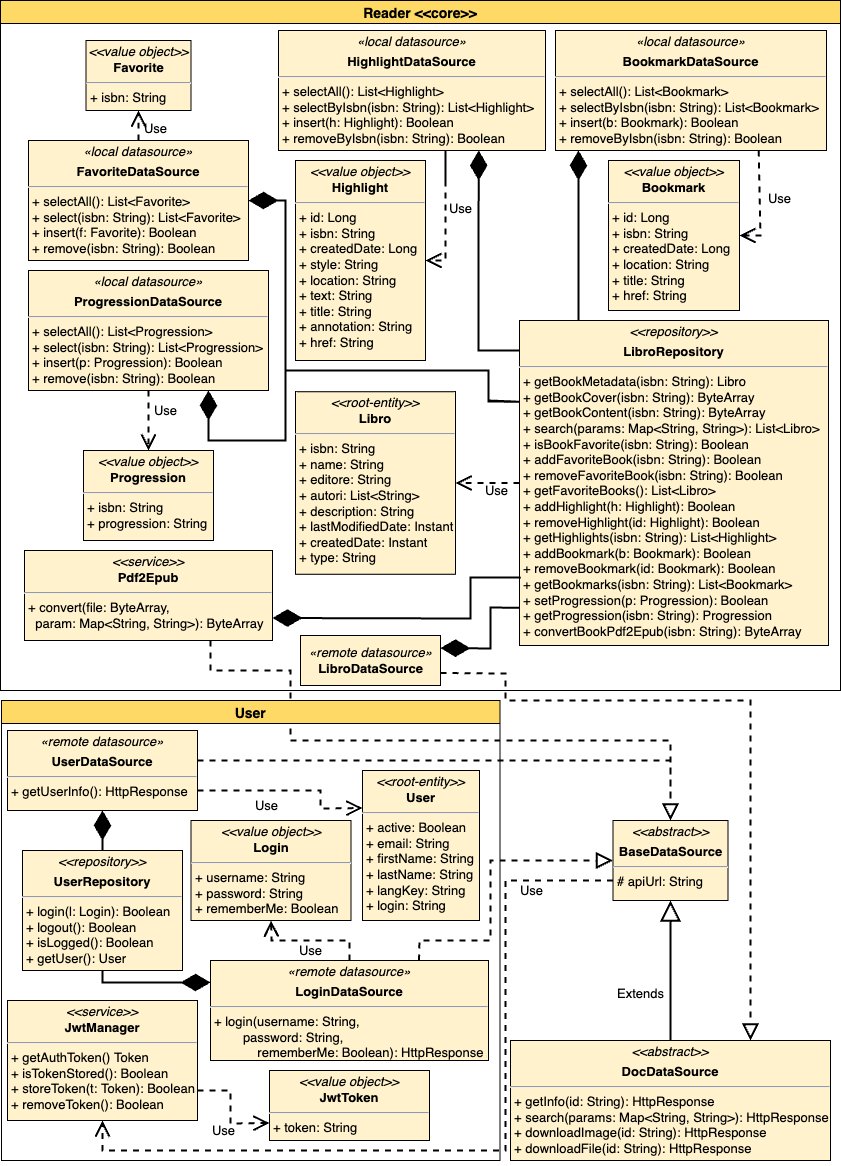
\includegraphics[width=1\textwidth]{img/class-uml-app.png}
        \caption{UML - Diagramma delle classi: Reader Core Domain e User Subdomain}
        \label{class-uml-app}
    \end{figure}
    
    \item \textbf{Aggregate} - Insieme di oggetti legati da una entità padre chiamata \textit{Root} (radice di aggregazione). L'aggregato composto da \textit{Bookmark}, \textit{Highlight}, \textit{Progression}, \textit{Favorite} ha come radice l'entità \textit{Libro}.
    \item \textbf{Service} - Operazione che non appartiene logicamente a nessun oggetto. In questo caso la conversione di formato non appartiene alla sola entità libro ma appartiene invece a qualsiasi documento che è possibile convertire.
    \item \textbf{Repository} - Oggetto per il recupero di altri oggetti di dominio e per la gestione del loro ciclo di vita. Le entità \textit{User} e \textit{Libro} sono esempi di oggetti di dominio che necessitano di un repository. Permette di disaccoppiare applicazione e domain design dalle specifiche tecnologie/strategie di persistenza come multipli database e datasource (locali e/o remoti).
\end{itemize}

\subsection{Progettazione UI/UX}
Successivamente alla modellazione del dominio e alla progettazione della architettura, le quali coinvolgono principalmente il modulo condiviso alle due applicazioni che si intende sviluppare grazie al framework KMM, è necessario progettare l'interfaccia grafica e l'esperienza utente che dovrà essere implementata invece per le rispettive piattaforme Android e iOS. Considerando l'utilizzo tipico di una applicazione con funzionalità simili a quella deve essere realizzata possono essere adottati pattern di navigazione e visualizzazione dei contenuti diventati oramai standard de-facto nella progettazione della UI/UX non solo per applicazioni mobile\footnote{\href{https://xd.adobe.com/ideas/principles/app-design/}{https://xd.adobe.com/ideas/principles/app-design/}}.

Alcuni esempi di questi elementi utilizzati sono il menu laterale a scomparsa (schermata 4), l'icona "hamburger" per l'apertura del menu (schermata 3),l' elenco di documenti con scroll infinito verticale (schermata 2-5) e la barra di ricerca nella parte alta della schermata con icona "lente di ingrandimento" (schermata 2-5). 

Per ottenere la validazione dei mockup da parte del committente sono state necessarie due iterazioni del processo di progettazione UX/UI. L'interfaccia utente desiderata deve infatti soddisfare alcuni vincoli caratteristici del brand Maggioli, come ad esempio l' utilizzo del colore blu \#00379E come colore primario, l'utilizzo del font Karla\footnote{\href{https://github.com/googlefonts/karla}{https://github.com/googlefonts/karla}} e la presenza del logo Maggioli.

Le schermate necessarie sono quindi: \textit{Reader}, responsabile della visualizzazione del contenuto digitale in formato EPUB; \textit{Login}, schermata iniziale responsabile alla autenticazione dell'utente; \textit{Home}, schermata principale responsabile alla visualizzazione dei contenuti digitali a cui l'utente è autorizzato ad accedere; \textit{Preferiti}, responsabile alla visualizzazione dei contenuti digitali preferiti dall'utente; \textit{Impostazioni}, responsabile alla visualizzazione e modifica delle impostazioni; \textit{About}, responsabile alla visualizzazione di informazioni generali come versione della applicazione, autore e copyright.

\begin{figure}[H]
    \centering
    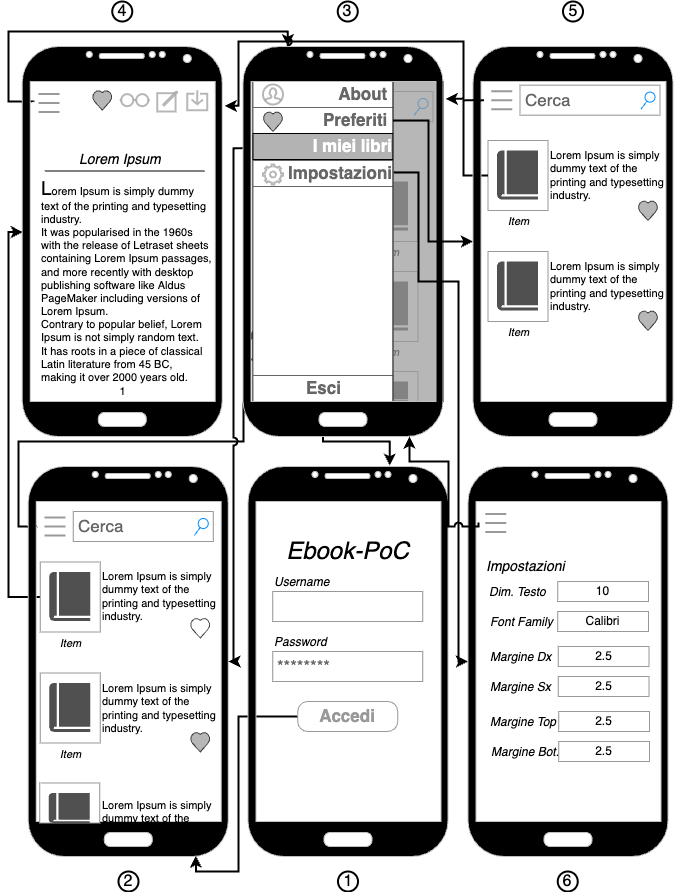
\includegraphics[width=1\textwidth]{img/mockup-uiux-1.png}
    \caption{Alcuni dei mockup realizzati per la progettazione e la validazione della UX/UI (prima iterazione)}
\end{figure}

\begin{figure}[H]
    \centering
    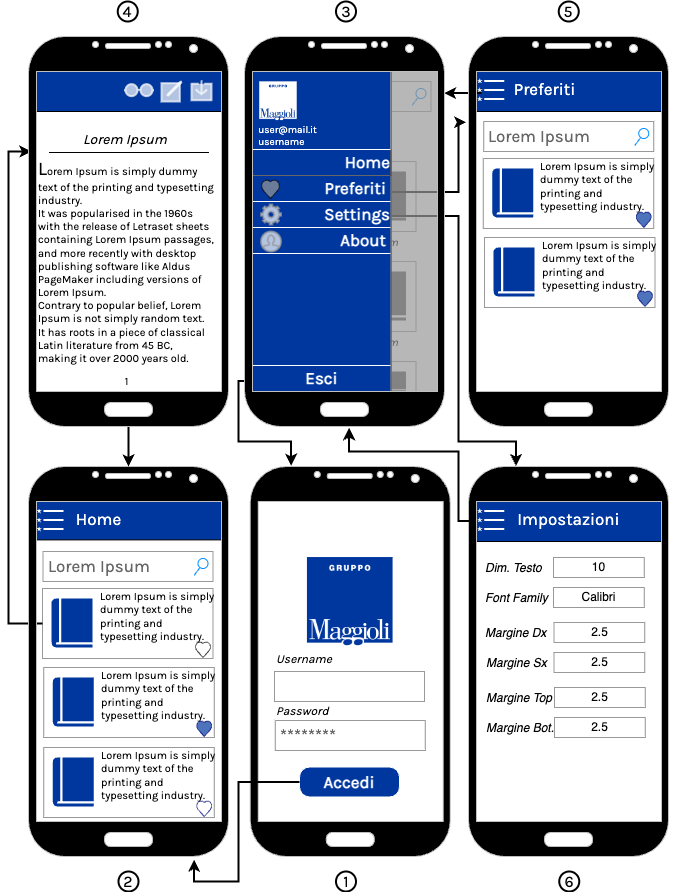
\includegraphics[width=1\textwidth]{img/mockup-uiux-2.png}
    \caption{Modifiche apportate ai mockup per ottenere la validazione della UX/UI (seconda iterazione)}
\end{figure}

\subsection{Architettura}
Lo scopo di una applicazione multipiattaforma è la condivisione della sola logica applicativa come mostrato nella struttura di un applicazione KMM (fig. \ref{stackKMM}). L'architettura in grado di supportare efficacemente questo concetto è conosciuta come \textit{Clean Architecture}~\cite{martin2017architecture} ed è composta da tre strati. Il primo strato (\textit{Data Layer}) consiste negli aggregati di dominio sopra descritti ed è responsabile per il recupero e il mantenimento dei dati su differenti sorgenti. Il secondo strato (\textit{Domain Layer}) facilità la comunicazione tra i differenti repository: qui si trovano tutti i casi d'uso del sistema che gestiscono il flusso dei dati provenienti o diretti verso il primo strato. Il terzo ed ultimo strato (\textit{View Layer}) si occupa della interfaccia grafica mostrando i dati e gestendo gli eventi provenienti dall'utente o dal sistema.

\begin{figure}[H]
    \centering
    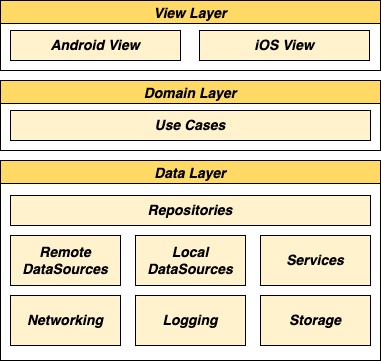
\includegraphics[width=0.6\textwidth]{img/clean-architecture.png}
    \caption{Clean Architecture in MaggioliEbook}
\end{figure}

\section{Sviluppo}
Tipicamente lo sviluppo effettivo di una applicazione multiplatform con il framework KMM ha inizio con la creazione dello scheletro della applicazione tramite l'IDE Android Studio e il relativo plugin Gradle KMM, come indicato nel capitolo \ref{ch:app-multiplatform}.

La prima attività successiva svolta in questa fase di sviluppo consiste nella ricerca delle librerie, definite dipendenze nel capitolo precedente. Considerando le funzionalità che devono essere implementate è necessario individuare tutte le librerie utili partendo da quelle core, come la visualizzazione e la modifica dei documenti, a quelle di utilità a supporto del modulo condiviso come networking e storage. Raggruppate per modulo di utilizzo, le librerie individuate e adottate sono:

\subsubsection*{Shared}
\begin{itemize} 
    \item \textbf{Ktor}\footnote{\href{https://github.com/ktorio/ktor}{https://github.com/ktorio/ktor}} - Framework asincrono per lo sviluppo di microservizi e applicazioni web, utilizzato per la parte di networking come client HTTP.
    \item \textbf{Kotlinx-Serialization} - Libreria multiplatform per la serializzazione dei dati.
    \item \textbf{Kotlinx-Datetime} - Libreria multiplatform per la gestione delle date e del tempo.
    \item \textbf{Kvault}\footnote{\href{https://github.com/Liftric/KVault}{https://github.com/Liftric/KVault}} - Libreria multiplatform per la persistenza dei dati sicura in formato chiave-valore. Tramite una unica API si comporta come wrapper di \textit{Keychain}, nel caso iOS, e \textit{SharedPreferences} nel caso Android.
    \item \textbf{Koin}\footnote{\href{https://github.com/InsertKoinIO/koin}{https://github.com/InsertKoinIO/koin}} - Dependency Injection framework multiplatform.
    \item \textbf{Napier}\footnote{\href{https://github.com/AAkira/Napier}{https://github.com/AAkira/Napier}} - Logging framework multiplatform.
    \item \textbf{SqlDelight}\footnote{\href{https://github.com/cashapp/sqldelight}{https://github.com/cashapp/sqldelight}} - Libreria multiplatform per la persistenza dei dati tramite database relazionale locale.
\end{itemize}

\subsubsection*{Android}
\begin{itemize}
    \item \textbf{Readium} (\textit{Kotlin-toolkit})\footnote{\href{https://github.com/readium/kotlin-toolkit}{https://github.com/readium/kotlin-toolkit}} - Libreria per la manipolazione e la visualizzazione di pubblicazioni digitali. Implementazione specifica per la piattaforma Android. 
\end{itemize}

\subsubsection*{iOS}
\begin{itemize}
    \item \textbf{Readium} (\textit{Swift-toolkit})\footnote{\href{https://github.com/readium/swift-toolkit}{https://github.com/readium/swift-toolkit}} - Libreria per la manipolazione e la visualizzazione di pubblicazioni digitali. Implementazione specifica per la piattaforma iOS. 
    \item \textbf{KMPNativeCoroutines}\footnote{\href{https://github.com/rickclephas/KMP-NativeCoroutines}{https://github.com/rickclephas/KMP-NativeCoroutines}} - Libreria che permette l'utilizzo delle coroutine Kotlin in Swift in applicazioni Kotlin Multiplatform.
\end{itemize}
    
\subsection{Readium}
La necessità di un tool open-source, robusto e performante per la manipolazione e la lettura di formati editoriali digitali è alla base del progetto Readium. Essa infatti consiste in un insieme di toolkit per diversi formati (come EPUB, audiolibri e libri image-based) e diverse piattaforme (Android, iOS, Desktop e Web).

L'architettura della libreria Readium è composta da quattro moduli principali:
\begin{itemize}
    \item \textbf{Publication Server} - Fornisce le pubblicazioni tramite un server locale HTTPS.
    \item \textbf{Streamer} - Modulo composto dai seguenti due sottomoduli:
    \begin{itemize}
        \item \textbf{Parser} - Responsabile del parsing delle pubblicazioni e della loro esposizione utilizzando un modello in-memory.
        \item \textbf{Fetcher} - Si occupa di ottenere i contenuti delle pubblicazioni e della loro manipolazione (in particolare injection di CSS e Javascript nelle risorse HTML).
    \end{itemize}
    \item \textbf{Navigator} - Utile alla navigazione delle risorse di una pubblicazione secondo diverse strategie basate sulla natura della pubblicazione (ebook, audiolibri, ...). Interagisce con il modulo \textit{Streamer} per utilizzare il modello in-memory o per ottenere manifesto JSON attraverso il modello condiviso (\textit{Shared}).
\end{itemize}

\begin{figure}[H]
    \centering
    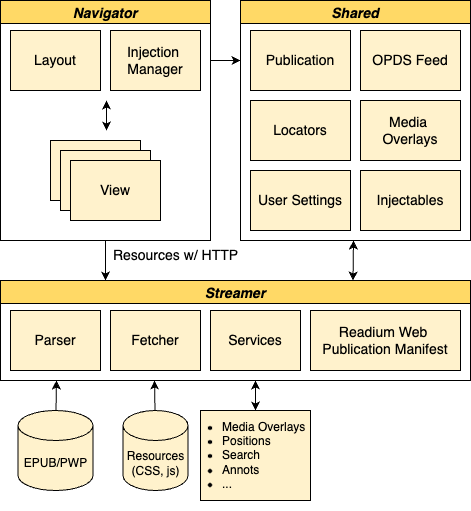
\includegraphics[width=0.75\textwidth]{img/readium-arch.png}
    \caption{Architettura libreria Readium}
    \label{readiumarch}
\end{figure}

\subsection{Modulo Shared}
% implementazione modulo shared


\subsection{Applicazione Android}
% implementazione app android

\subsection{Applicazione iOS}
% implementazione app iOS
